\documentclass[UTF8]{resume}

\name{邱江坤}
\address{\faPhone~+86 158 6659 6952 \faEnvelope~\href{mailto://qiujiangkun@foxmail.com}{qiujiangkun@foxmail.com} \faGithub~\href{https://github.com/qiujiangkun/}{GitHub: qiujiangkun} \faWeixin~同手机号 ~~~~~}
\address{实习目标: 后端开发}


\begin{document}

\begin{tikzpicture}[remember picture, overlay] 
    \node[anchor = north east] at ($(current page.north east)+(-1.3cm,-1.2cm)$) {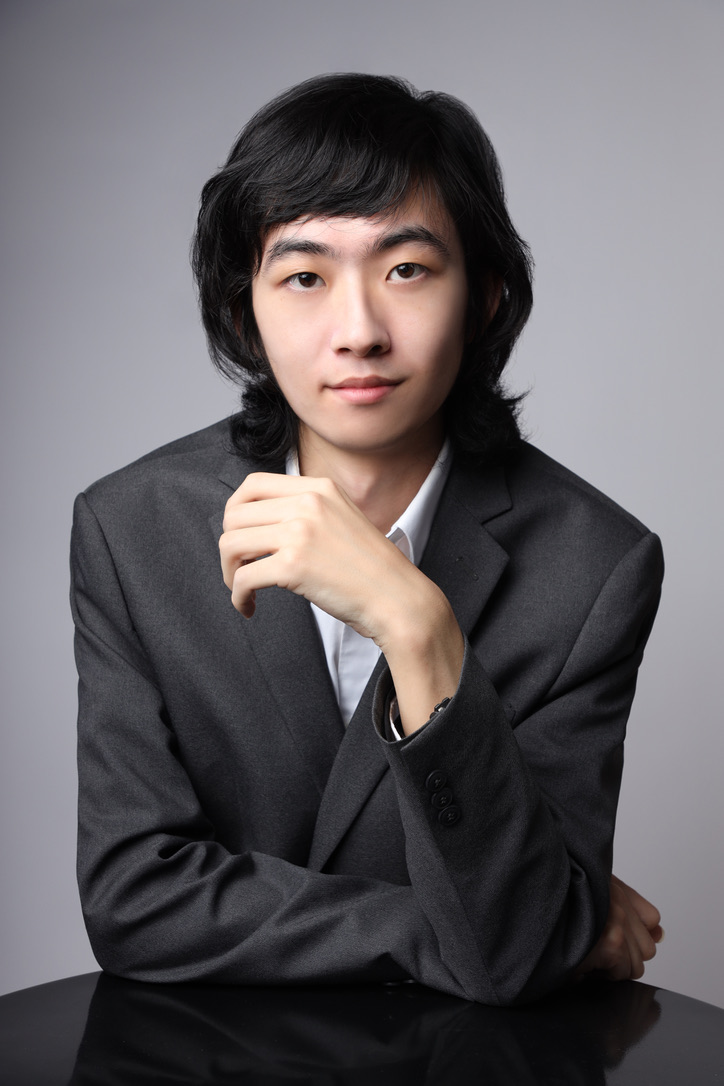
\includegraphics[height=2.5cm]{avatar.jpg}};
  \end{tikzpicture}
  

\begin{rSection}{\faCogs~编程经验}
    \begin{itemize}
        \itemsep -0.5em \vspace{-0.5em}
        \item 9年编程经验,热衷开源,能够独自或合作编写上万行代码的项目
        \item 熟悉C++、Java、Python、Rust、Scala; 了解JavaScript、Bash、SQL、C\#、PHP、汇编
        \item 熟悉Linux, git、计算机底层、机器学习、深度学习;了解Kafka、K8S、Netty、Disruptor、并发编程、JVM调优、编译原理
    \end{itemize}
    
\end{rSection}
\begin{rSection}{\faGraduationCap~教育经历}
    \begin{itemize}
        \item 香港科技大学~综合系统与设计(编程方向)专业\hfill 2020.9-今
    \end{itemize}
\end{rSection}

\begin{rSection}{\faBriefcase~工作经历}
    \begin{rExperience}{软件开发实习生}{麦穗人工智能~上海穰川信息技术有限公司}{2020.12-今}
        \textbf{实习内容}
        \begin{itemize}
            \itemsep -0.5em \vspace{-0.5em}
            \item 搭建分布式限流器:利用Akka和Redis和经过修改过的滑动日志法,搭建分布式限流器,针对每个用户和每个API限速,解决了经过ingress负载均衡后各节点上Akka Stream无法将流量限制到较小的数目的问题
            \item 对接企业微信应用:用Python开发企业微信第三方应用原型,打通智能招聘的添加联系方式和发放招聘资料环节
            \item 低速刷新服务:从PostgreSQL读取变更日志,清洗出每个租户的变更数据,根据每个租户限速配置,写入不同Kafka topics;实现供运维使用的低速刷新任务队列和Web控制台,以受限SQL注入的形式配置低速刷新任务队列
        \end{itemize}
    \end{rExperience}
    \begin{rExperience}{软件开发工程师}{数字货币交易公司(保密)}{2020.07-今}
        \textbf{项目背景}:
        升级现有客户端并发网络库,降低交易网站信息收集处理数据延迟,编写高频交易的底层库\\
        \textbf{项目内容}
        \begin{itemize}
            \itemsep -0.5em \vspace{-0.5em}
            \item 搭建网络库:使用Rust语言,运用缓存行优化和无锁队列等底层优化,实现客户端并发的网络库,并支持多种通信协议;通过修改Webpki和Rustls等库,支持对IP地址的TLS的链接;以极低的延迟从不同的交易平台收集并处理数据;正在构建基于f-stack的用户态网络库;基于UDP实现转发器,绕开服务器机房对于IP的限制;支持Arm架构和x86架构
            \item 搭建监控系统:运用InfluxdDB和Grafana搭建监控系统,实时监控不同交易平台数据采集处理情况
            \item 搭建绘图引擎:修改Matplotlib,支持大量数据的实时绘图,同时兼容Matplotlib所有的特性
            \item 搭建分布式回测系统:搭建K8S回测集群,利用kafka和PostgreSQL完成回测系统的数据输入和收集
            \item 实现JSON解析库:用过程宏、CPU缓存、减少缺页错误和数据特征,将JSON反序列化效率提高到原来8倍,快于Serde库一倍
            \item 项目成果:总延迟与Apache Benchmark持平,测试环境数据明显优化及提升
        \end{itemize}
    \end{rExperience}
\end{rSection}

% TODO:做更好的项目
% TODO:根据公司切换项目
\begin{rSection}{\faUsers~项目经历}
    % \begin{rProject}{个人项目}{Minecraft 服务器}{2020.10-今}
    %     \textbf{项目概述}:开发兼容Minecraft客户端的高性能服务器后台\\
    %     \textbf{开发原因}:现有的Minecraft服务器单机支持的客户端数量较低,因此希望开发一款支持高在线人数的服务器\\
    %     \textbf{项目开发}:使用Scala开发,除去协议部分,完全自己重写,正在开发
    % \end{rProject}

    \begin{rProject}{合作项目}{WP-Reliable MD}{2018.09-2019.10}
        \textbf{项目概述}:某Markdown插件的原作者停止开发,于是将Markdown编辑器Tui-Editor成功引入WordPress插件商店\\
        \textbf{项目职责}
        \begin{itemize}
            \itemsep -0.5em \vspace{-0.5em}
            \item 项目管理:担任组长,带领3开发团队,完成整体架构设计、技术选型和早期开发
            \item 项目开发:使用JavaScript,针对WordPress的界面风格设计了GUI,并替换掉编辑器的渲染引擎,重写渲染模块,使其支持Tex数学公式。采用非侵入式的方法,避免造成文章内容丢失和内容不一致。
        \end{itemize}
        \textbf{项目成果}:多人采用WP-Reliable MD作为博客的编辑器
    \end{rProject}

    % \begin{rProject}{个人项目}{Escape射击游戏}{2020.02}
    %     \textbf{项目概述}:作为AI的训练环境和体验游戏,2D鸟瞻视角射击游戏项目\\
    %     \textbf{游戏设计}:该游戏需要大量AI互动,需要一定的物理特效和性能需求\\
    %     \textbf{项目开发}:游戏主打功能性,用C++17开发,采用Entt ECS框架,Box2D作为物理引擎,LUA作为脚本引擎,使用模板和多态开发序列化库,极大提升了C++开发能力
    % \end{rProject}

    % \begin{rProject}{个人项目}{英语文章阅读器}{2019.04}
    %     \textbf{项目概述}:帮助非英语母语在网站上阅读英语文章时,查阅单词,生成背诵表而开发的网页端应用\\
    %     \textbf{功能设计}:主要功能包含全文翻译,选词翻译和自动查询功能,可以导出单词表和标记掌握的词汇\\
    %     \textbf{项目开发}:使用Python Flask作为后端,前端采用Semantic UI和jQuery
    % \end{rProject}

    % \begin{rProject}{个人项目}{卓信社交平台}{2018.08}
    %     \textbf{项目概述}:仿照Facebook和Penpal World开发的简单的社交平台\\
    %     \textbf{功能设计}:用户注册、登录、关联QQ、发帖、关注、个人资料编辑、广场、搜索用户、后台\\
    %     \textbf{项目开发}:采用的技术有PHP,HTML,JavaScript,MySQL,Semantic UI
    % \end{rProject}
\end{rSection}

\begin{rSection}{\faAward~获奖经历~资格认证}
    \begin{itemize}
        \itemsep -0.5em \vspace{-0.5em}
        \item 托福英语考试~总分106(听力29,阅读30,口语21,写作26) \hfill 2019.10
        \item 中国计算机学会~认证学生会员 \hfill 2019.07
        \item RoboCom机器人大赛全球锦标赛~一等奖 \hfill 2018.07
        \item 清华大学登峰杯数据挖掘竞赛~二等奖 \hfill 2018.07 
        \item 全国计算机等级考试~四级网络工程师 \hfill 2016.11
        \item 第19届中国移动“和”教育杯电脑制作大赛~一等奖(项目第一名) \hfill 2016.07
    \end{itemize}
\end{rSection}
\end{document}
